\chapter{Конструкторский раздел}

Для проектирования программной реализации необходимо разбить весь процесс на этапы. При разбиении следует руководствоваться теми или иными, уже существующими, решениями для хранения и обработки информации.

В данной работе под коллекцией документов здесь и далее понимается массив новостей на русском языке. В сети Интернет документы хранятся в виде html-файлов.
Для обучения модели необходимо получить данные в виде мешков слов.
Кроме того, из-за большого объема данных необходимо разделить предварительную обработку каждого документа и последующий сбор обработанных данных в общую коллекцию для обучения.

Отдельным пунктом была рассмотрена структура анализируемых данных, чтобы при выборе средств реализации можно было использовать эту информацию. 

Процесс создания тематической модели разбивается на следующие этапы:

\begin{itemize}
    \item сбор данных;
    \item обработка данных;
    \item обучение модели;
    \item использование модели;
    \item оценка модели.
\end{itemize}


%
\section{Структура анализируемых данных}

Очевидно, что для работы решения необходимо хранить коллекцию новостей, где о каждом документе известны тема новости, текст новости, ссылка на html-файл новости в сети Интернет.

Так как данные обрабатываются подокументно, будет удобно иметь данные в обработанном виде рядом с сырыми, чтобы иметь возможность обрабатывать коллекцию по частям.

При описании структуры данных желательно предоставить возможность обновлять данные, так как со временем html документы на выбранном ресурсе могут меняться. Для этого необходимо хранить дату сохранения документов.

Кроме того, процесс обработки данных также может быть усовершенствован или изменен. Следовательно, также необходимо хранить дату обработки данных.

Так как все данные текстовые и однородные, для хранения выбрана таблица в базе данных со следующими полями: 

\begin{itemize}
    \item тема новости;
    \item текст новости; 
    \item ссылка на html файл новости в сети Интернет;
    \item обработанный текст новости;
    \item дата сохранения документа;
    \item дата обработки данных.
\end{itemize}

~\

Для организации сохранения всех новостей с выбранного ресурса необходимо отслеживать на какие страницы ресурса ведут уже обработанные страницы. Для этого создается еще одна таблица с данными: какая ссылка, на какую другую ссылку ведет. То есть создается таблица со следующими полями: 

\begin{itemize}
    \item ссылка-родитель;
    \item ссылка-ребенок.
\end{itemize}

~\

Ограничения:

\begin{itemize}
    \item Новости на русском языке.
\end{itemize}

%
\section{Сбор данных}


В аналитическом разделе были выделены несколько типов данных: 

\begin{itemize}
    \item предварительно подготовленные массивы новостей; 
    \item новостные сайты;
    \item новостные агрегаторы.
\end{itemize}

~\

Рассмотрим их детальнее. 

%
\subsubsection{Предварительно подготовленные массивы новостей}

Обычно в таких массивах данных текст новостей и их заголовки уже очищены от форматирования и переносов, опечатки исправлены, а также удалена нетекстовая информация. При этом остаются следующие проблемы:

\begin{itemize}
    \item слишком короткие тексты;
    \item слова в новостях не приведены к нормальной форме;
    \item не выделены словосочетания;
    \item много часто используемых слов и редко используемых слов;
    \item каждый такой массив данных оформлен по-своему, поэтому для работы с ним необходимо писать код, преобразующий коллекцию в удобный для модели формат.
\end{itemize}
 

Так как часть обработки уже выполнена, получить такой массив данных предпочтительнее, чем добывать данные из сети Интернет. Но стоит учесть, что найти такие массивы данных достаточно сложно. Необходимо опрашивать специалистов в этой области, изучать платформы сообществ по обработке естественного языка, анализировать архивы конференций.

%
\subsubsection{Новостные сайты и агрегаторы}

У данных, хранящихся в сети Интернет, существует большое количество недостатков: они не обработаны, текст хранится вперемешку с html кодом, содержит опечатки. Также из-за неорганизованности владельцев новостных сайтов, зачастую важные для последующего анализа данные (например, дата публикации, имя документа и т.д.) хранятся в разном виде за разные периоды времени, и поэтому их сложно извлечь. 

С другой стороны, такой подход предоставляет практически безграничные возможности выбора тематики для последующего анализа.

Для извлечения таких данных необходим специальный софт, который анализирует указанный интернет ресурс, а также все ссылки, на которые ведут уже скачанные страницы. Отдельно стоит отметить,и что часть ссылок зачастую на новостных сайтах появляются динамически, после того, как посетитель сайта нажимает специальную кнопку или перематывает страницу до конца.

Также учитывая технические ограничения автора работы и то, что документов на выбранном ресурсе может быть много, необходимо, чтобы процесс анализа и сохранения новостей можно было остановить в любой момент и впоследствии продолжить с места остановки.

Так как данная задача довольно распространена существует библиотеки, частично или полностью решающие проблему получения данных. Однако, часто данные на сайтах хранятся в таком виде, что приходится модифицировать существующие решения. 

%
\section{Обработка данных}

После того, как получены сырые данные, перед началом обучения модели, данные необходимо подготовить. Подготовка данных разбивается на два этапа:

\begin{itemize}
    \item обработка документа (новости);
    \item формирование коллекции в формате, удобном для модели.
\end{itemize}

%
\subsubsection{Обработка документа (новости)}

В рамках этого этапа подготовки данных производится обработка по документам. В связи с техническими ограничениями необходим хранить дату обработки, чтобы иметь возможность при изменении алгоритма выполнить процесс подготовки текста повторно. Кроме того, так же, как и в случае с сохранением страницы сети Интернет, из-за того, что данных много, необходимо реализовать возможность подготовки новостей коллекции по частям, останавливая и запуская процесс в любой момент времени.

Подготовку данных по документам можно разбить на следующие этапы.

\begin{itemize}
    \item\textbf{Очистка от форматирования и переносов.} В сыром виде текст новости часто перемешан с html кодом, специальными символами pdf файлов, часть слов разделены дефисов для переноса на новую строку.
    \item\textbf{Исправление опечаток.} Журналисты и редакторы могут не уследить за орфографической ошибкой, и обучаемая модель воспримет слово с ошибкой как отдельное редкое слово в коллекции.
    \item\textbf{Удаление нетекстовой информации:} рисунков, графиков, таблиц.
    \item\textbf{Приведение слов к нормальной форме.} Для английского языка используется \textbf{стемминг} (выделение неизменной части слова). Для данной работы лучше подходит \textbf{лемматизация}, так как новости на русском языке.
    \item\textbf{Выделение словосочетаний.} По умолчанию модель воспринимает каждое слово в тексте новости как отдельный термин. При выделении словосочетаний появляется возможность, обучая модель, относиться к ним как к цельным многословным терминам.
    \item\textbf{Удаление часто используемых слов.} Часто используемые слова встречаются в большом количестве тем, и их наличие в документе не может стать признаком того, какие именно темы затрагиваются в новости. 
    \item\textbf{Удаление редко используемых слов.} Редко используемые слова (обычно встречающиеся меньше десяти раз за коллекцию) также не несут обычно никакой информации о принадлежности документа к той или иной теме.
\end{itemize}

%
\subsubsection{Формирование коллекции в формате, удобном для модели}

После того, как каждый документ обработан и представлен в виде мешка слов необходимо собрать все документы в одну коллекцию. В связи с техническими ограничениями потребуется возможность собирать такую коллекцию по частям на основании источника документа, даты скачивания, даты обработки. В зависимости от выбранной реализации модели так же следует привести данные в формат, необходимый для обучения модели. Конкретное представление данных выбрано в технологическом разделе. Формирование коллекции должно выполняться отдельно от обработки подокументно так как происходит непосредственно перед обучением модели и может зависеть от целей исследователя.

%
\section{Обучение модели}

Согласно выбранному алгоритму сначала модель обучается на подготовленных данных без регуляризаторов (как в рассматриваемом варианте алгоритма PLSA) до того момента как перплексия перестанет изменяться. Это будет означать, что слова достаточно хорошо и однозначно распределились по темам и осталась только задача тематизирования документов.

После этого в модель добавляются регуляризаторы по одному. Добавляя регуляризатор исследователь подбирает параметры регуляризатора, там образом, что бы перплексия уменьшалась, разреженность матриц $\Phi$ и $\Theta$ увеличивалась, но при этом, что бы не достигала единицы. То же самое касается остальных параметров. Частота тем должна стремиться к величине равное количество слов, поделенное на количество тем.

В данной работе были рассмотрены три регуляризатора. Ниже приводятся их формальные описания и интерпретации. В первых двух регуляризаторах реч идет о разреживании или сглаживании, так как при положительных коэффициентах $\tau$ при соответствующих регуляризаторах значения матриц сглаживаются, а при отрицательных разреживаться.

Разреживающий или сглаживающий регуляризатор матрицы слово-тема $\Phi$:
$$
R(\Phi) = \tau \sum_{t \in T}{ \sum_{w \in W} \ln{ \phi_{wt} }} \rightarrow max.
$$

Разреживающий или сглаживающий регуляризатор матрицы тема-документ $\Theta$:
$$
R(\Theta) = \tau \sum_{d \in D}{ \sum_{t \in T} \ln{ \theta_{td} }} \rightarrow max.
$$

Максимизация регуляризатора декоррелирования тем приводит к тому, что темы как столбцы матрицы $\Phi$ как можно меньше коррелируют друг с другом:
$$
R(\Phi) = -{{\tau}\over{2}} \sum_{t \in T}{ 
    \sum_{s \in T\\t}{
        \sum_{w \in W}{
            \phi_{wt} \phi_{ws}
        }
    }
} \rightarrow max.
$$

После анализа функционала решения была разработана диаграмма метода (рисунки \ref{fig:IDEF0_1} и \ref{fig:IDEF0_2}).

\begin{figure}[h]
    \center{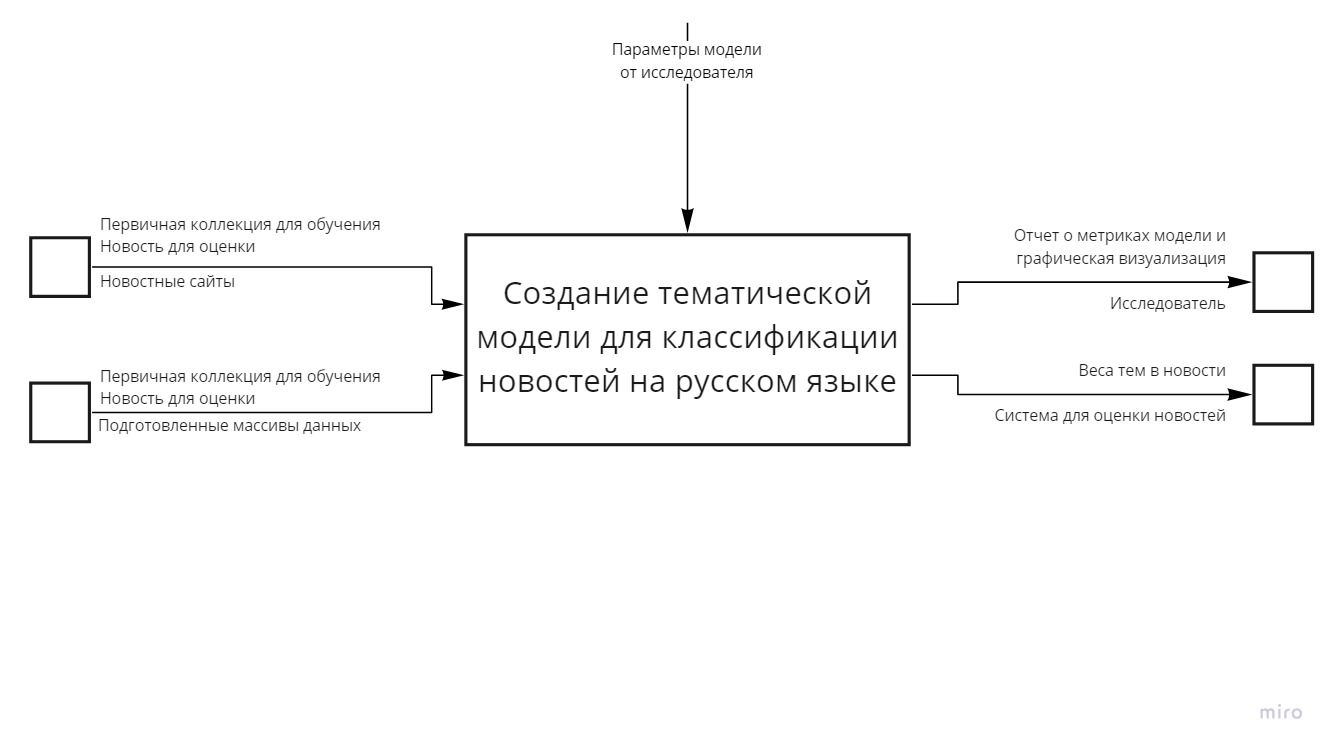
\includegraphics[scale=0.3]{A0.jpg}}
    \caption{Диаграмма метода 1}
    \label{fig:IDEF0_1}
\end{figure}

\begin{figure}[h]
    \center{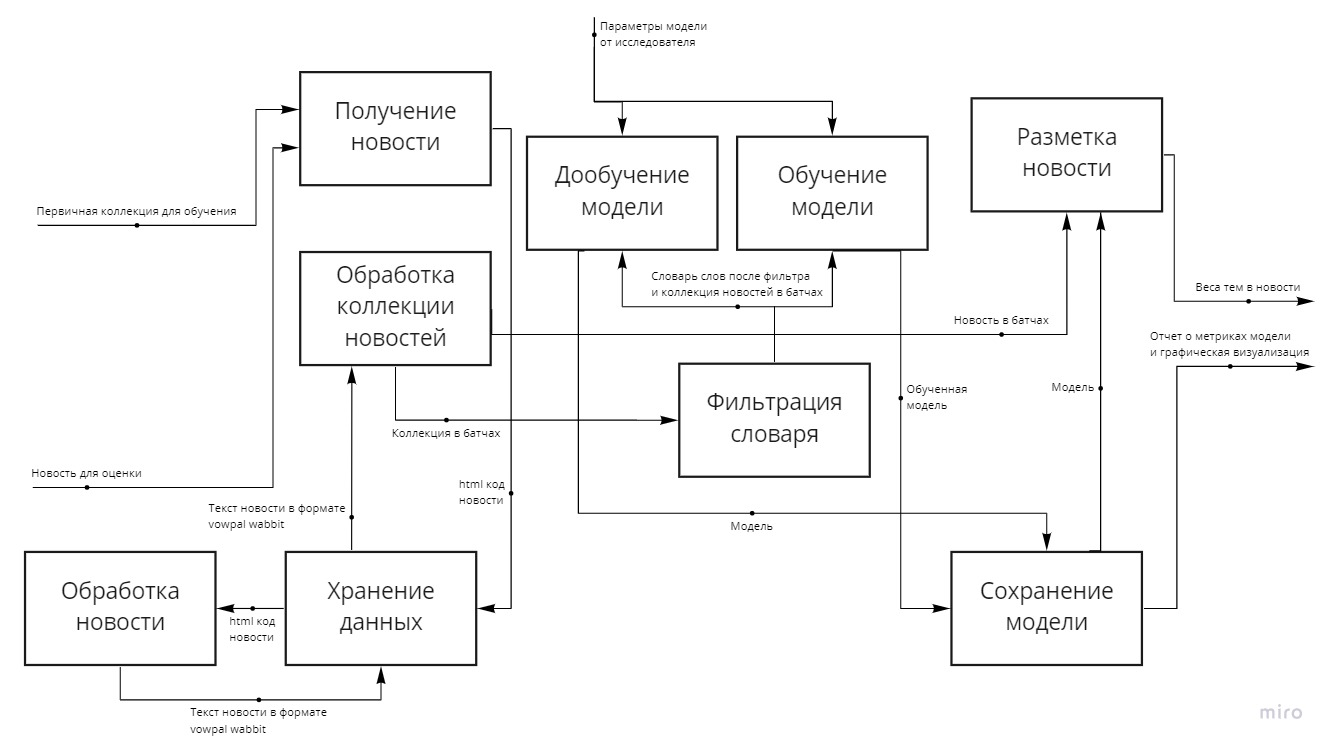
\includegraphics[scale=0.3]{A1.jpg}}
    \caption{Диаграмма метода 2}
    \label{fig:IDEF0_2}
\end{figure}
    
%
\section{Использование модели}

При выборе реализации алгоритма в технологической части необходимо удостовериться, что любую построенную модель можно сохранить, а также загрузить в дальнейшем для последующего использования.

После загрузки модели, также должна быть возможность дообучения, чтобы сократить время на создание сложных моделей, также необходим функционал по оценке нового документа (новости) с помощью загруженной модели.
%
\section{Оценка модели}

Для оценки полученных результатов были использованы следующие метрики:

\begin{itemize}
    \item перплексия;
    \item разреженность матрицы слово-тема $\Phi$;
    \item разреженность матрицы тема-документ $\Theta$;
    \item средний контраст тем;
    \item средняя чистота тем;
    \item средний размер тем;
    \item 10 наиболее вероятных слов в теме.
\end{itemize}

Меньшая перплексия чаще всего означает, что темы более интерпретируемы, но сама по себе эта метрика ничего не значит. Она принимает значения от нуля до бесконечности и подходит только для сравнения моделей на дном и тех же данных, с одним и тем же количеством тем. Перплексия вычисляется по следующей формуле:
$$
P(D;\Phi,\Theta) = \exp{\big( 
    -{{1}\over{n}} \sum_{d \in D}{
        \sum_{w \in d}{
            n_{dw} \ln{
                \sum_{t \in T}{
                    \phi_{wt} \theta_{td}
                }
            }
        }
    } 
\big)}.
$$

Разреженность матрицы слово-тема $\Phi$ изменяется от 0 до 1 и интерпретируется как процент значений в матрице $\Phi$ близких к нулю. Чем ближе значение этой метрики к единице, тем меньшим количеством слов описана тема и тем лучше становится интерпретируемость тем.

Разреженность матрицы тема-документ $\Theta$ изменяется от 0 до 1 и интерпретируется как процент значений в матрице $\Theta$ близких к нулю. Чем ближе значение этой метрики к единице, тем меньшим количеством тем описан документ и тем лучше становится интерпретируемость тем.

Следующие три метрики строятся на основании ядра темы. Пусть ядро темы определяется следующей формулой:
$$
W_t = \{
    w \in W|p(t|w) > 0
\}
$$

Чев выше контраст у темы, тем меньше будет пересечений. То же самое справедливо для средней величины по всем темам. Контраст темы определяется формулой:
$$
{{1}\over{|W_t|}}\sum_{w \in W_t}{
    p(t|w)
}
$$

Чем выше чистота темы, тем легче человека ее интерпретировать. То же самое справедливо для средней величины по всем темам. Данная метрика определяется формулой:
$$
\sum_{w \in W_t}{
    p(w|t)
}
$$

Средний размер тем определяется значением $|W_t|$ и в оптимальном случае стремится к отношению количества слов в коллекции к количеству тем.

10 наиболее вероятных слов в теме необходимы для того, что бы проверить интерпретируемость тем исследователем.

Так же для того, что бы облегчить анализ данных исследователю, при разработке решения необходимо написать процедуру вывода графического представления рассмотренных выше статистик.

%
\section{Требования к реализации}

На основании проведенного анализа в конструкторской части были сформированы следующие требования к реализации:

\begin{itemize}
    \item необходимо использовать реляционную базу данных для хранения документов,
    \item необходимые сущности и поля в базе данных:
    \begin{itemize}
        \item сущность страницы:
        \begin{itemize}
            \item тема новости,
            \item текст новости,
            \item ссылка на html-файл новости в сети Интернет,
            \item обработанный текст новости,
            \item дата сохранения документа,
            \item дата обработки данных;
        \end{itemize}
        \item сущность ссылки:
        \begin{itemize}
            \item ссылка родитель,
            \item ссылка ребенок;
        \end{itemize}
    \end{itemize}
    \item программный комплекс должен состоять из следующих отдельных процедур:
    \begin{itemize}
        \item сбор информации
        \item обработка информации подокументно
        \item формирование коллекции для обучения
        \item обучение модели
        \item использование модели
        \item вывод параметров модели для оценки
    \end{itemize}
    %\item при сборе данных необходимо указывать дату сохранения html-файла
\end{itemize}